\subsection*{Sistema de detección de rostro y reconocimiento de gestos para robot animatrónico}
Anteriormente en la Universidad del Valle de Guatemala (UVG), el estudiante Luis Eduardo Ruano Argueta trabajó un software para la detección del rostro y emociones. Para este proyecto se utilizó Python, OpenCV, Base de datos de rostros, entre otros. Se utilizan dos algoritmos distintos para clasificar las distintas emociones y ellos utilizan una cámara Logitech 920 para obtener las imágenes en tiempo real \cite{Ruano2019Tesis}.

El objetivo principal de este proyecto es implementar por medio de software un programa que pueda darle seguimiento a los rostros y el reconocimiento de expresiones faciales de las personas. Para esto se realizó una comparación entre dos algoritmos. Uno que utiliza algoritmos en cascada y otro que utiliza las marcas de cara. Se analizaron ambos algoritmos en dos ambientes diferentes, uno controlado y uno no controlado para evaluar el desempeño de ambos en aspectos como la distancia máxima, movimientos laterales, agresividad de movimientos y rotación con respecto al ángulo de visión. Entre los resultados destaca el alcance máximo del algoritmo \textit{Haar cascade}, con un alcance máximo de 5.31m en ambientes controlados y abiertos. Mientras que el algoritmo de marcas de cara destaca en cuando a la detección cuando existe un ángulo de rotación mayor a 45°al ángulo de visión respecto a la cámara. \cite{Ruano2019Tesis}.

Los algoritmos seleccionados para el \textit{Haar cascade} y el algoritmo de marcas de cara son \textit{Fisher Face} y SVM respectivamente. Para el algoritmo \textit{Fisher Face} se realizó reconstrucción de imágenes y representación de estas por medio de dispersión de datos. Para el algoritmo SVM se utilizó marcas de cara para generar entrenamientos \cite{Ruano2019Tesis}.

Para las bases de datos se utilizó una base de datos descargada llamada \textit{Cohn-Kanade} y las bases generadas \textit{UVG}, \textit{UVG 2m}, \textit{Ambiente 2} y \textit{Personalizada}. Estas bases de datos se utilizaron para entrenar los algoritmos para trabajar en los distintos ambientes, ya sean controlados  o no, cantidad de iluminación, distancia, entre otros \cite{Ruano2019Tesis}.

Se tuvieron problemas al momento de reconocer ciertas expresiones, ya que los algoritmos las confundian con otras. Al realizar las pruebas se limitó la cantidad de expresiones para detectar a 3: Feliz, enojo y sorpresa. Al realizar esta modificación se tuvo una mejora en los resultados teniendo un porcentaje de éxito por encima del 68\%, donde el más bajo fue de 68.21\% para el ambiente UVG 2m con el algoritmo \textit{Fisher Face} \cite{Ruano2019Tesis}.

\begin{figure}[h]
    \centering
    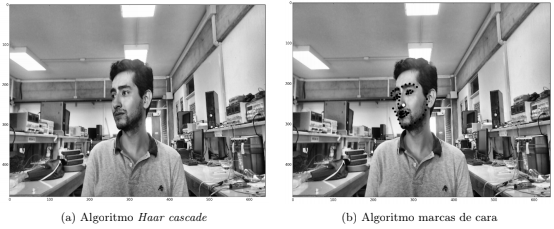
\includegraphics[width=0.7\textwidth]{figuras/Ruano_Result.png}
    \caption{Detección de rostros con angulo de visión de 45°. \cite{Ruano2019Tesis}}
    \label{fig:RuanoResult}
\end{figure}

\newpage
\subsection*{Detector de emociones utilizando OpenCV}
El usuario de medium.com, Karan  Sethi, publicó un artículo donde presenta el procedimiento y resultados de la deteccion de sus rostro y el reconocimiento de 5 emociones. El usuario utilizó el software de OpenCV para la visión por computadora y Keras para el aprendizaje automático. El procedimiento que utilizó se reduce en dos grandes etapas, la creación del modelo, que incluye el entrenamiento del mismo, y la implementación del modelo para el reconocimiento de emociones en tiempo real \cite{Karan}.

En el artículo, Karan, dice explicitamente que los prerrequisitos para poder realizar este proyecto es tener conocimiento básico de los sigueintes temas:
\begin{itemize}
\item Python
\item OpenCV
\item Red neuronal de convolución (CNN)
\item numpy
\end{itemize}

El objetivo principal de Karan es crear una red neuronal de convolución utilizando Keras, la API para Python sobre (\textit{Deep Learning}), para detectar emociones en tiempo real a través de la realimentación al sistema de una cámara en tiempo real \cite{Karan}.

Para esto, él realiza la primera etapa, la creación del modelo, en cinco tareas. La primera tarea es importar todos los módulos necesarios en el proyecto, declarar algunas variables como la cantidad de emociones, los pixeles de las imágenes que se estarán utilizando y la cantidad de muestras que se tomarán antes de que el modelo se actualice. Seguido de eso, realiza la segunda tarea, la cual es importar el \textit{dataset} que se estará utilizando. Él utiliza el \textit{dataset} de \textbf{fer2013}, un \textit{dataset} de libre uso alojado en la plataforma de \textbf{kaggle}. Este contiene siete clases, las cuales corresponden a las siete emociones básicas, sin embargo, karan utiliza solo cinco de esas clases. Ahora continuamos con la tercera tarea la cual consiste en expandir el \textit{dataset} que se está utilizando de manera artificial. Para esto utiliza \textbf{Keras}, que tiene la capacidad de ajustar modelos usando la clase . Ahora, la cuarta tarea es crear el cerebro de nuestro modelo, es decir, la CNN. Se define el modelo que se estará utilizando que, en el caso de Karan, es el modelo secuencial que define que todas las capas en la red serán secuenciales y las alamcenará en una variable del modelo. Por último, la quinta tarea es compilar y entrenar el modelo. Para esto se importan algunas librerías, se crean algunas funciones y luego se compila y ajusta el modelo. Con esto ya solo quedaría implementar el modelo para el reconocmiento de emociones en tiempo real \cite{Karan}.

Ahora, Karan, realiza la segunda etapa. La cual consta de crear el driver para usar el modelo creado anteriormente. Lo primero es importar algunos módulos necesarios para el funcionamiento del código, como las herramientas de OpenCV. También hay que cargar el modelo y el algoritmo de clasificación, él utiliza \textbf{Haar Cascade} que es una algortimo para identificar objetos en imágenes o videos. Después de programar y terminar el código el detector de emociones estaría terminado. Y como resultado se tendría lo mostrado en la Figura \ref{fig:KaranResult} \cite{Karan}.

\begin{figure}[h]
    \centering
    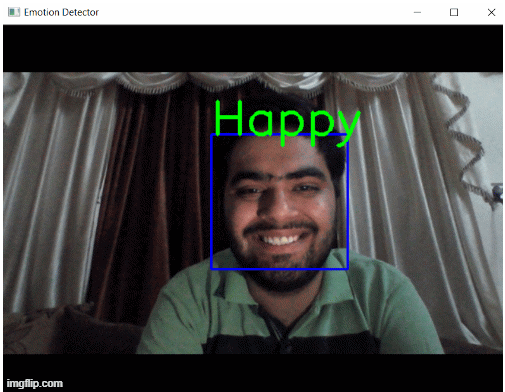
\includegraphics[width=0.5\textwidth]{figuras/Karan_Result.png}
    \caption{Resultado del detector de emociones de Karan Sethi. \cite{Karan}.}
    \label{fig:KaranResult}
\end{figure}